\section{Zero-shot Classification Examples}
\label{app:lit}

\Cref{tab:lit_examples} contains example zero-shot classifications of generated images.
These images were provided by the Parti~\citep{parti} and Imagen~\citep{imagen} models.
The training data for the ViT-22B vision backbone and the LiT text backbone was created before these models were trained, therefore these images are not present in the training data. 
Further, the objects and scenes contained in these images are highly out-of-distribution relative to the distribution of natural images on the web.

\begin{figure}[hb]
\newlength{\figwidth}\setlength{\figwidth}{0.45\textwidth}
\centering
\resizebox{0.92\columnwidth}{!}{%
\begin{tabularx}{\textwidth}{ cc }
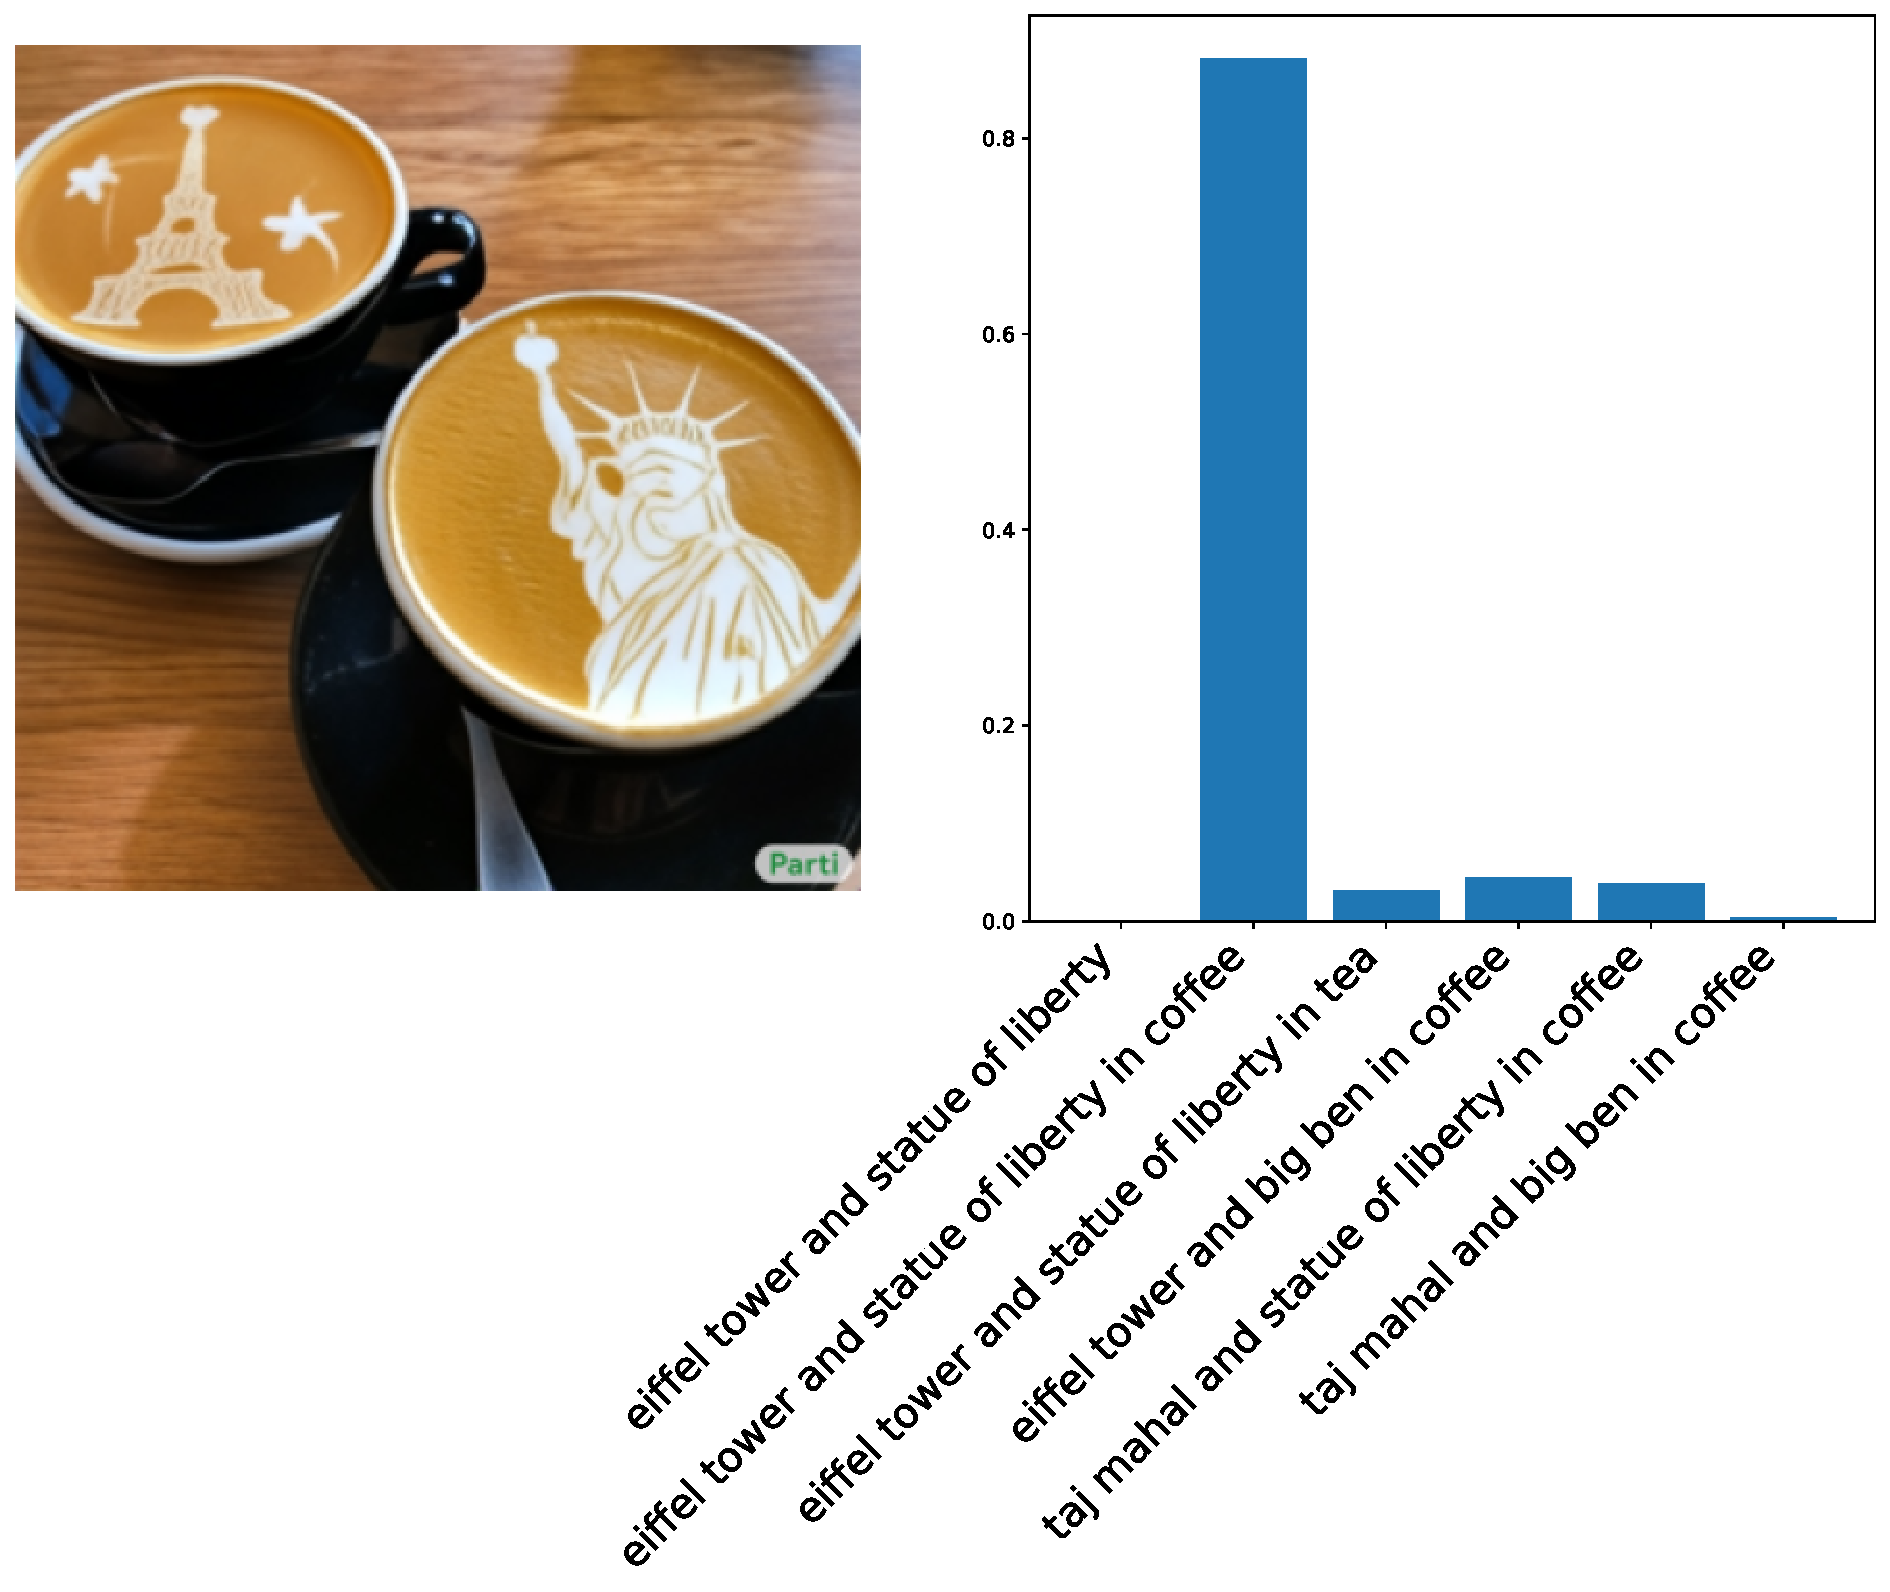
\includegraphics[width=\figwidth,valign=t]{figs/lit-1.pdf} &
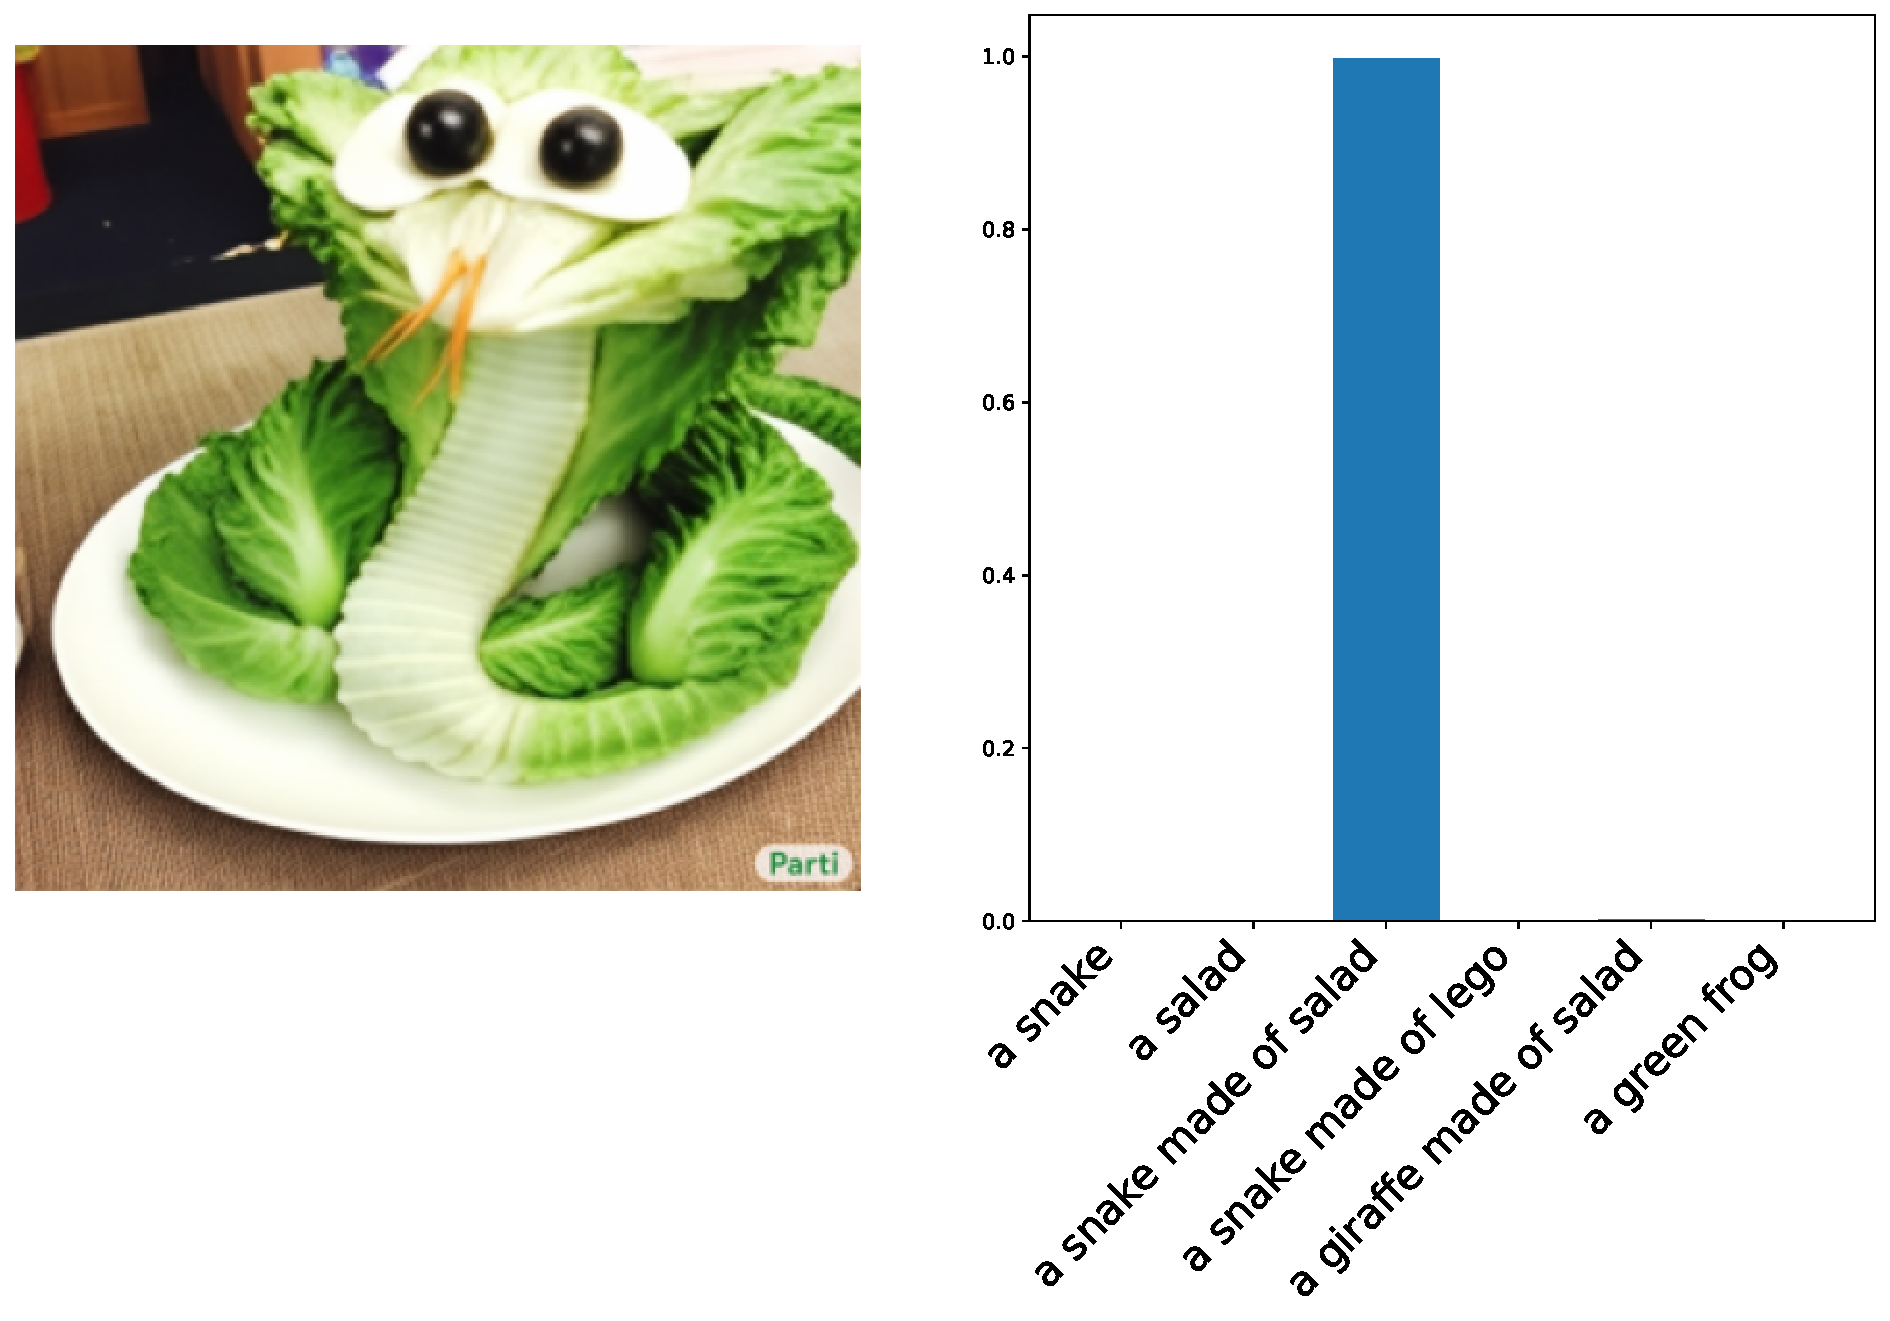
\includegraphics[width=\figwidth,valign=t]{figs/lit-2.pdf}\\
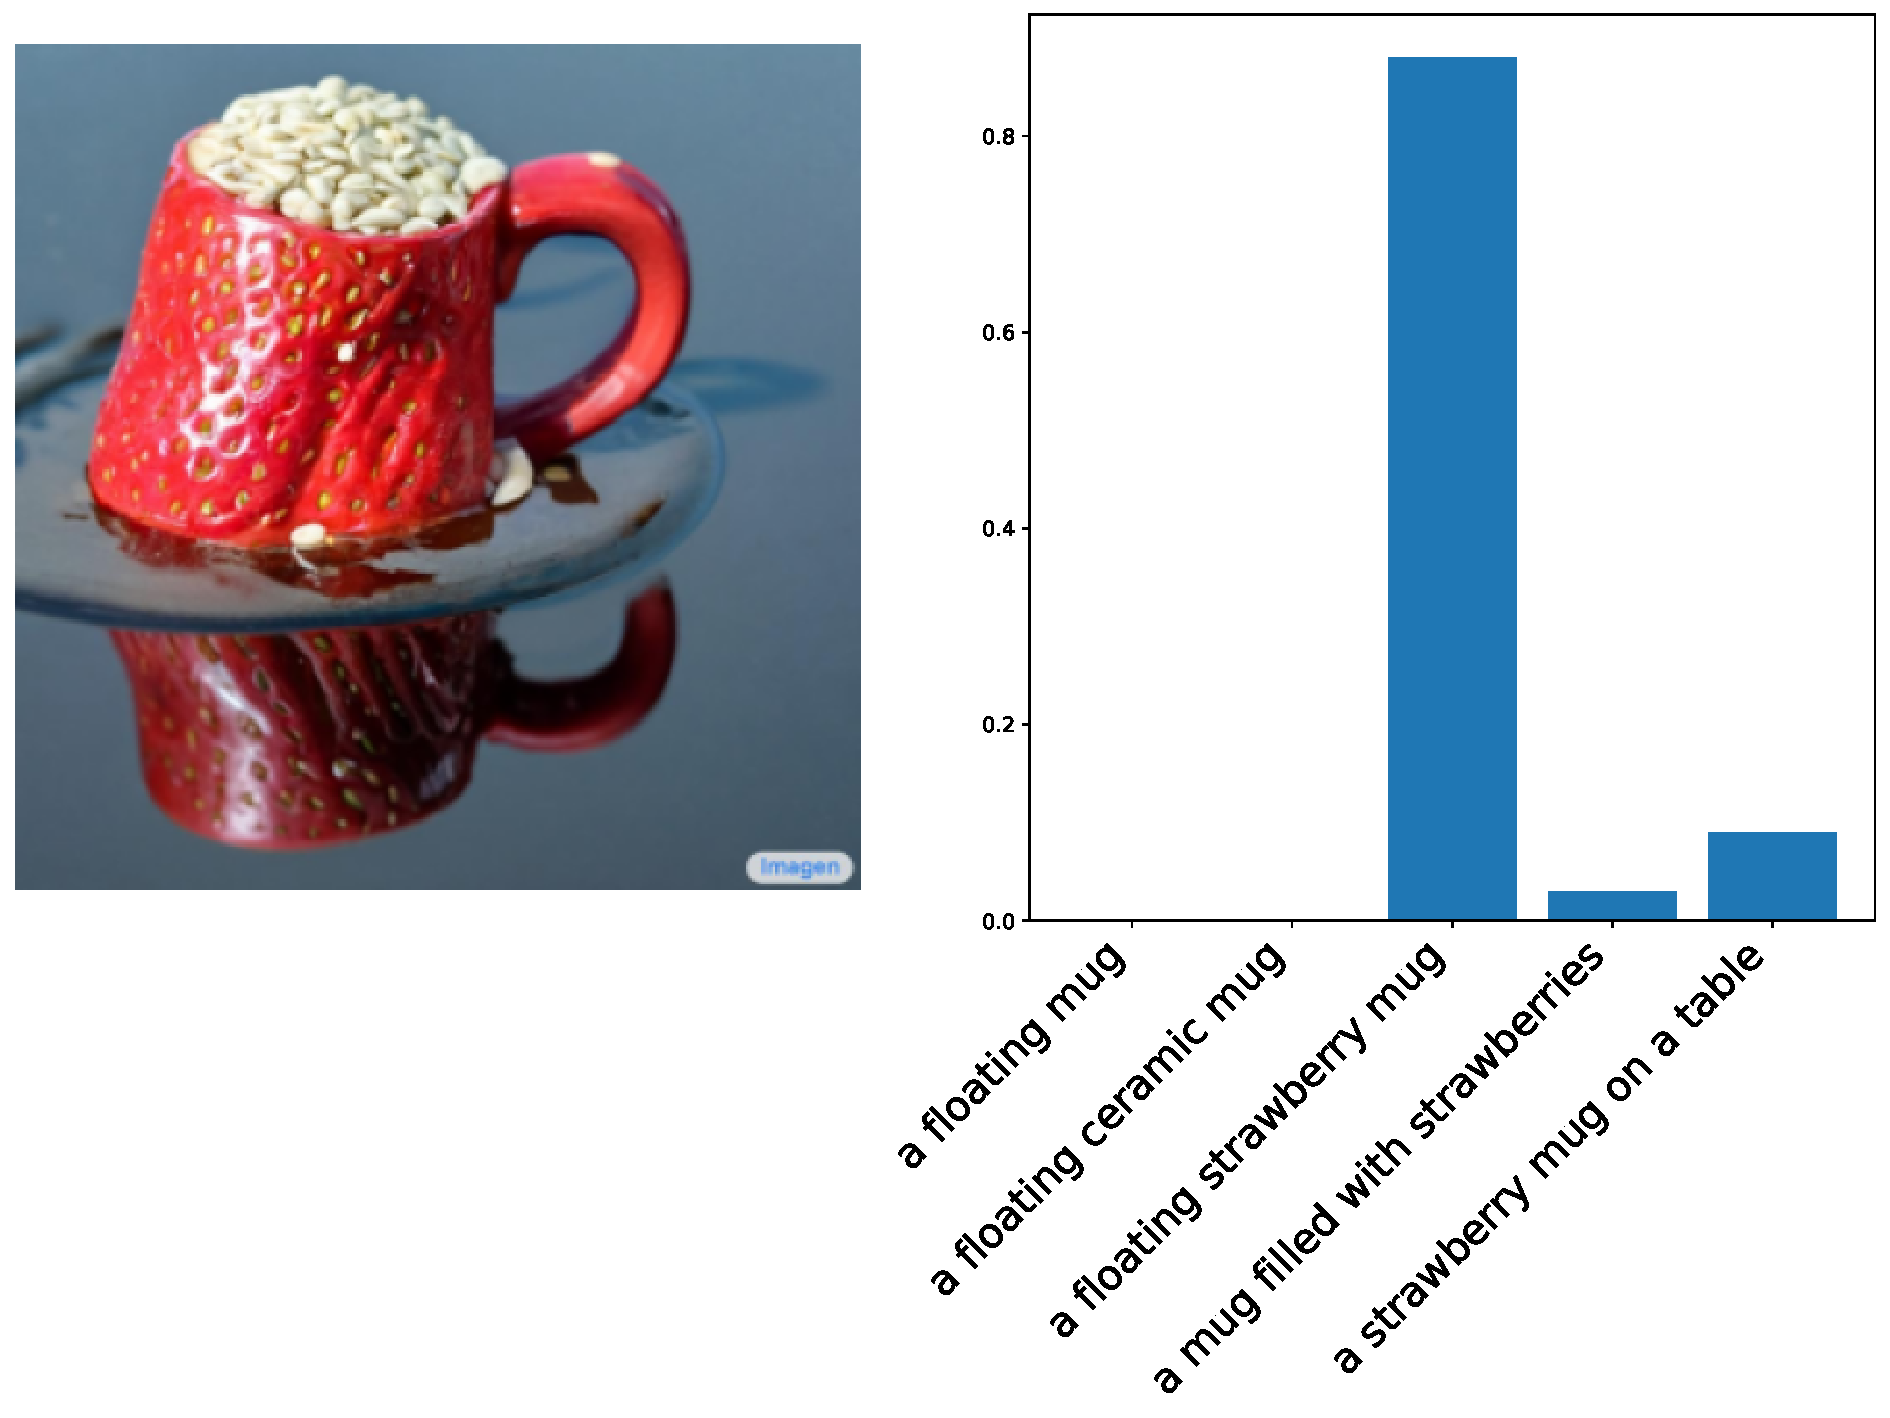
\includegraphics[width=\figwidth,valign=t]{figs/lit-3.pdf} &
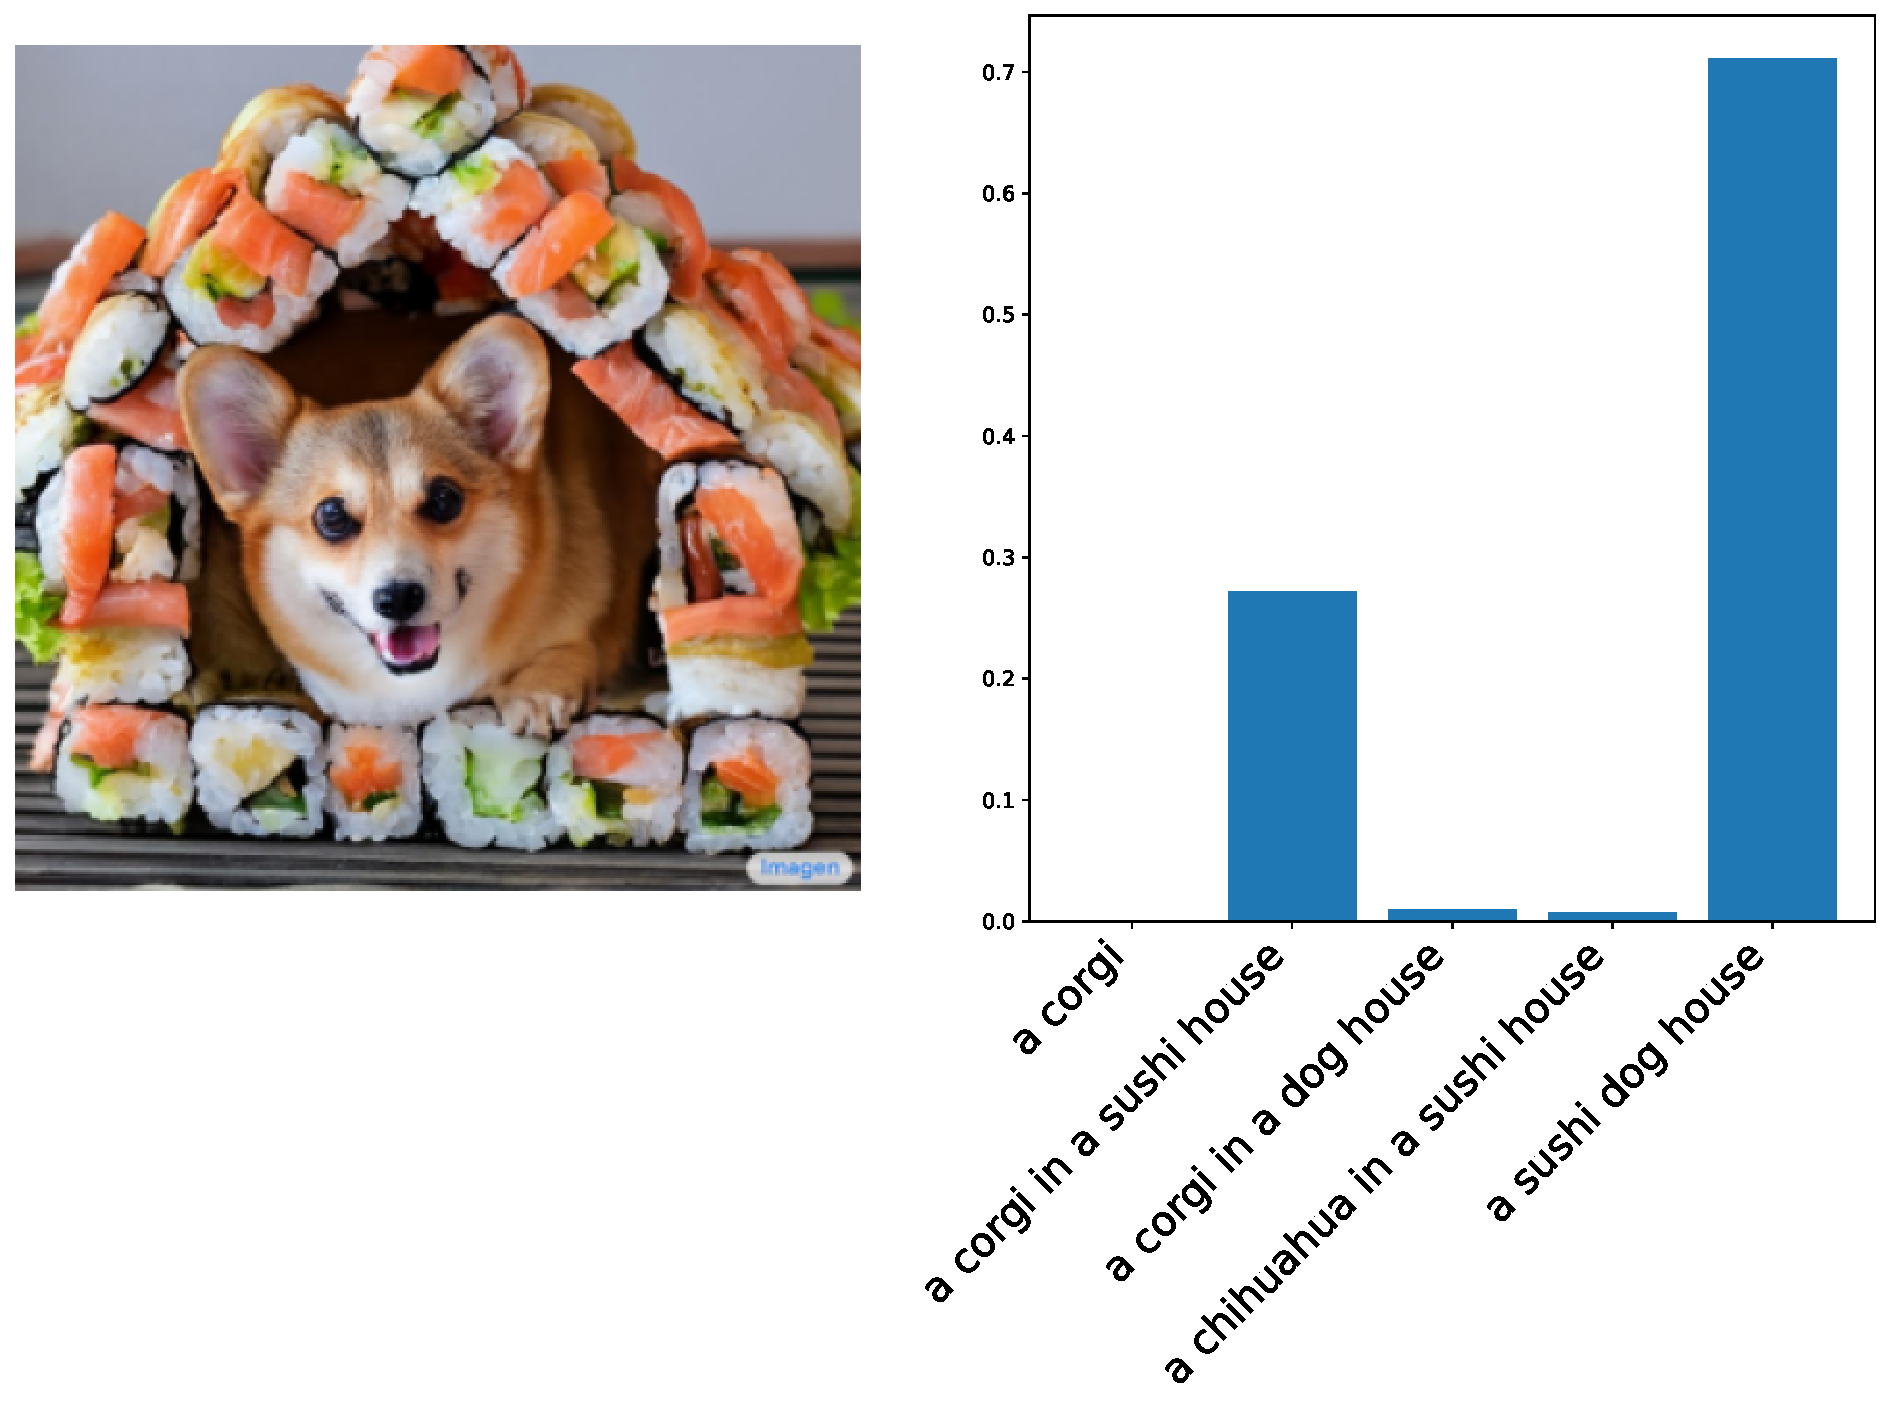
\includegraphics[width=\figwidth,valign=t]{figs/lit-4.pdf}\\
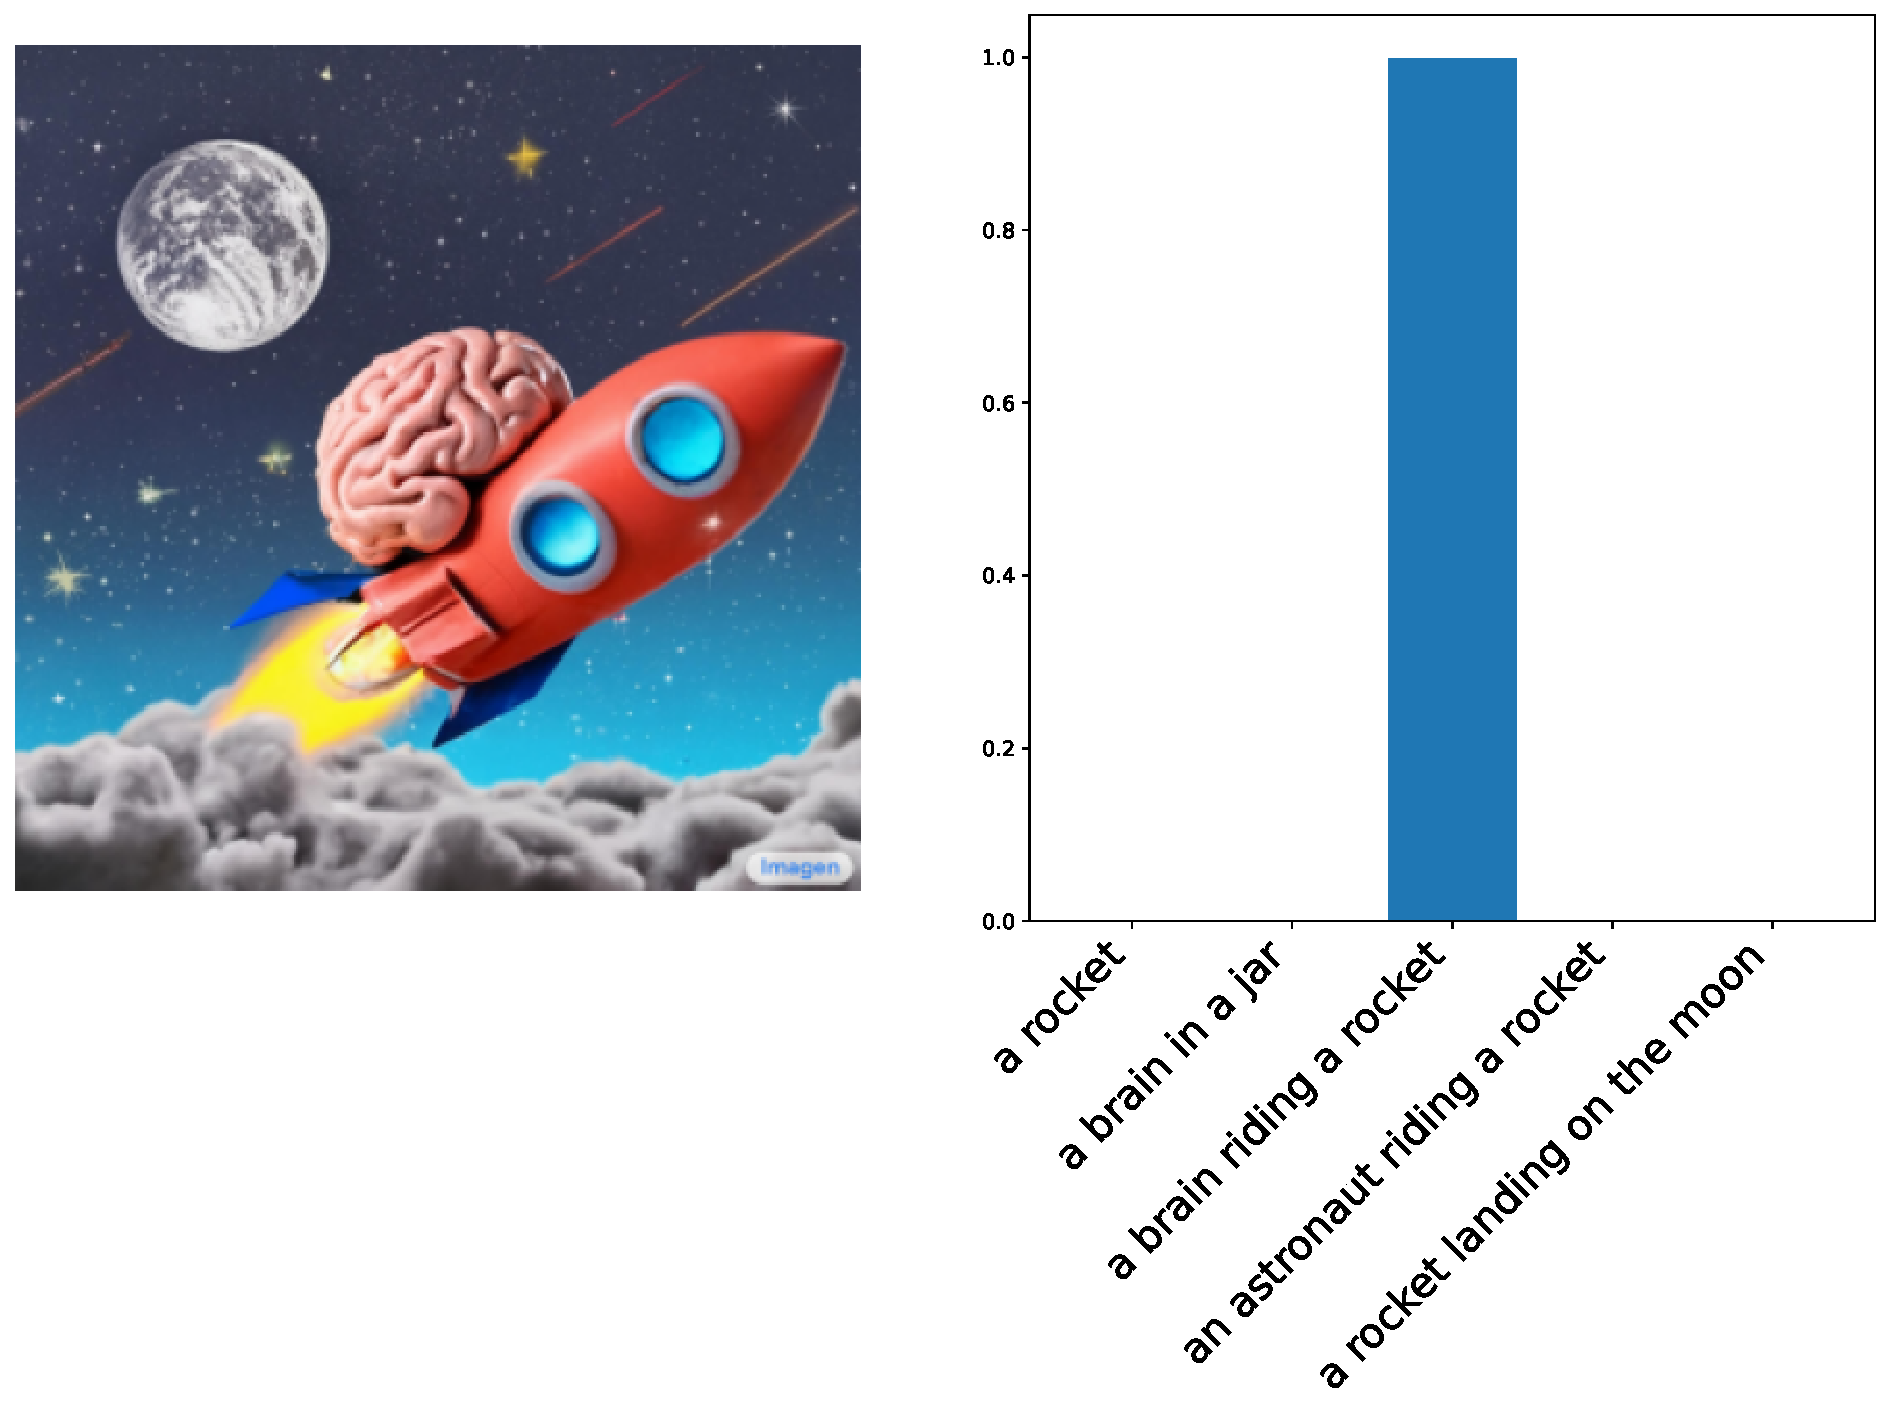
\includegraphics[width=\figwidth,valign=t]{figs/lit-5.pdf} &
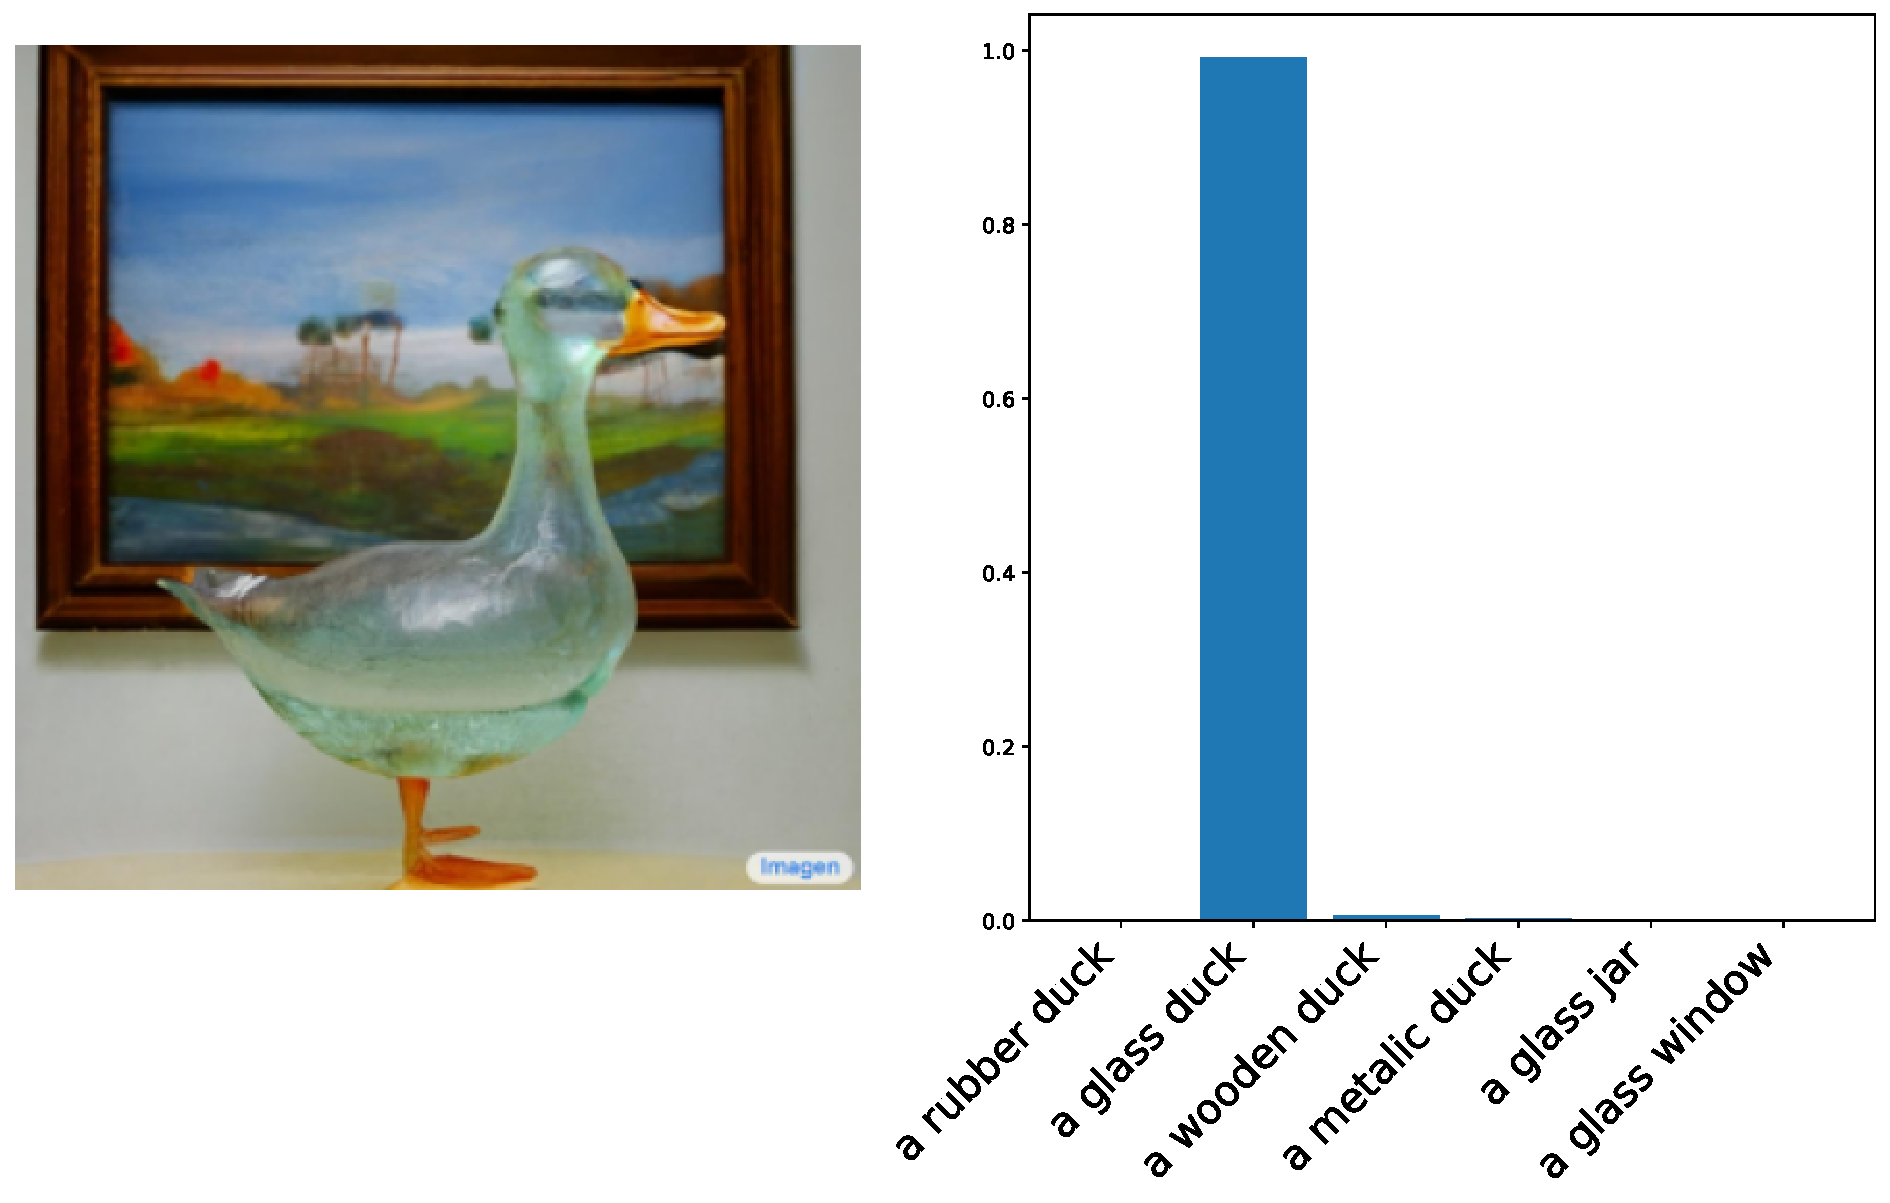
\includegraphics[width=\figwidth,valign=t]{figs/lit-6.pdf}\\
\end{tabularx}%
} %close resizebox
\caption{Examples of zero-shot classification results on images generated by the Parti~\citep{parti} and Imagen~\citep{imagen} models.
These examples contain unusual objects/scenes that do not occur in the training distribution.
\label{tab:lit_examples}
}
\end{figure}
\clearpage
\newpage